\chapter{Algorithms and Indices}

\section{Sorting Algorithms (unassessed)}
\subsection{Quicksort}
\begin{center}
    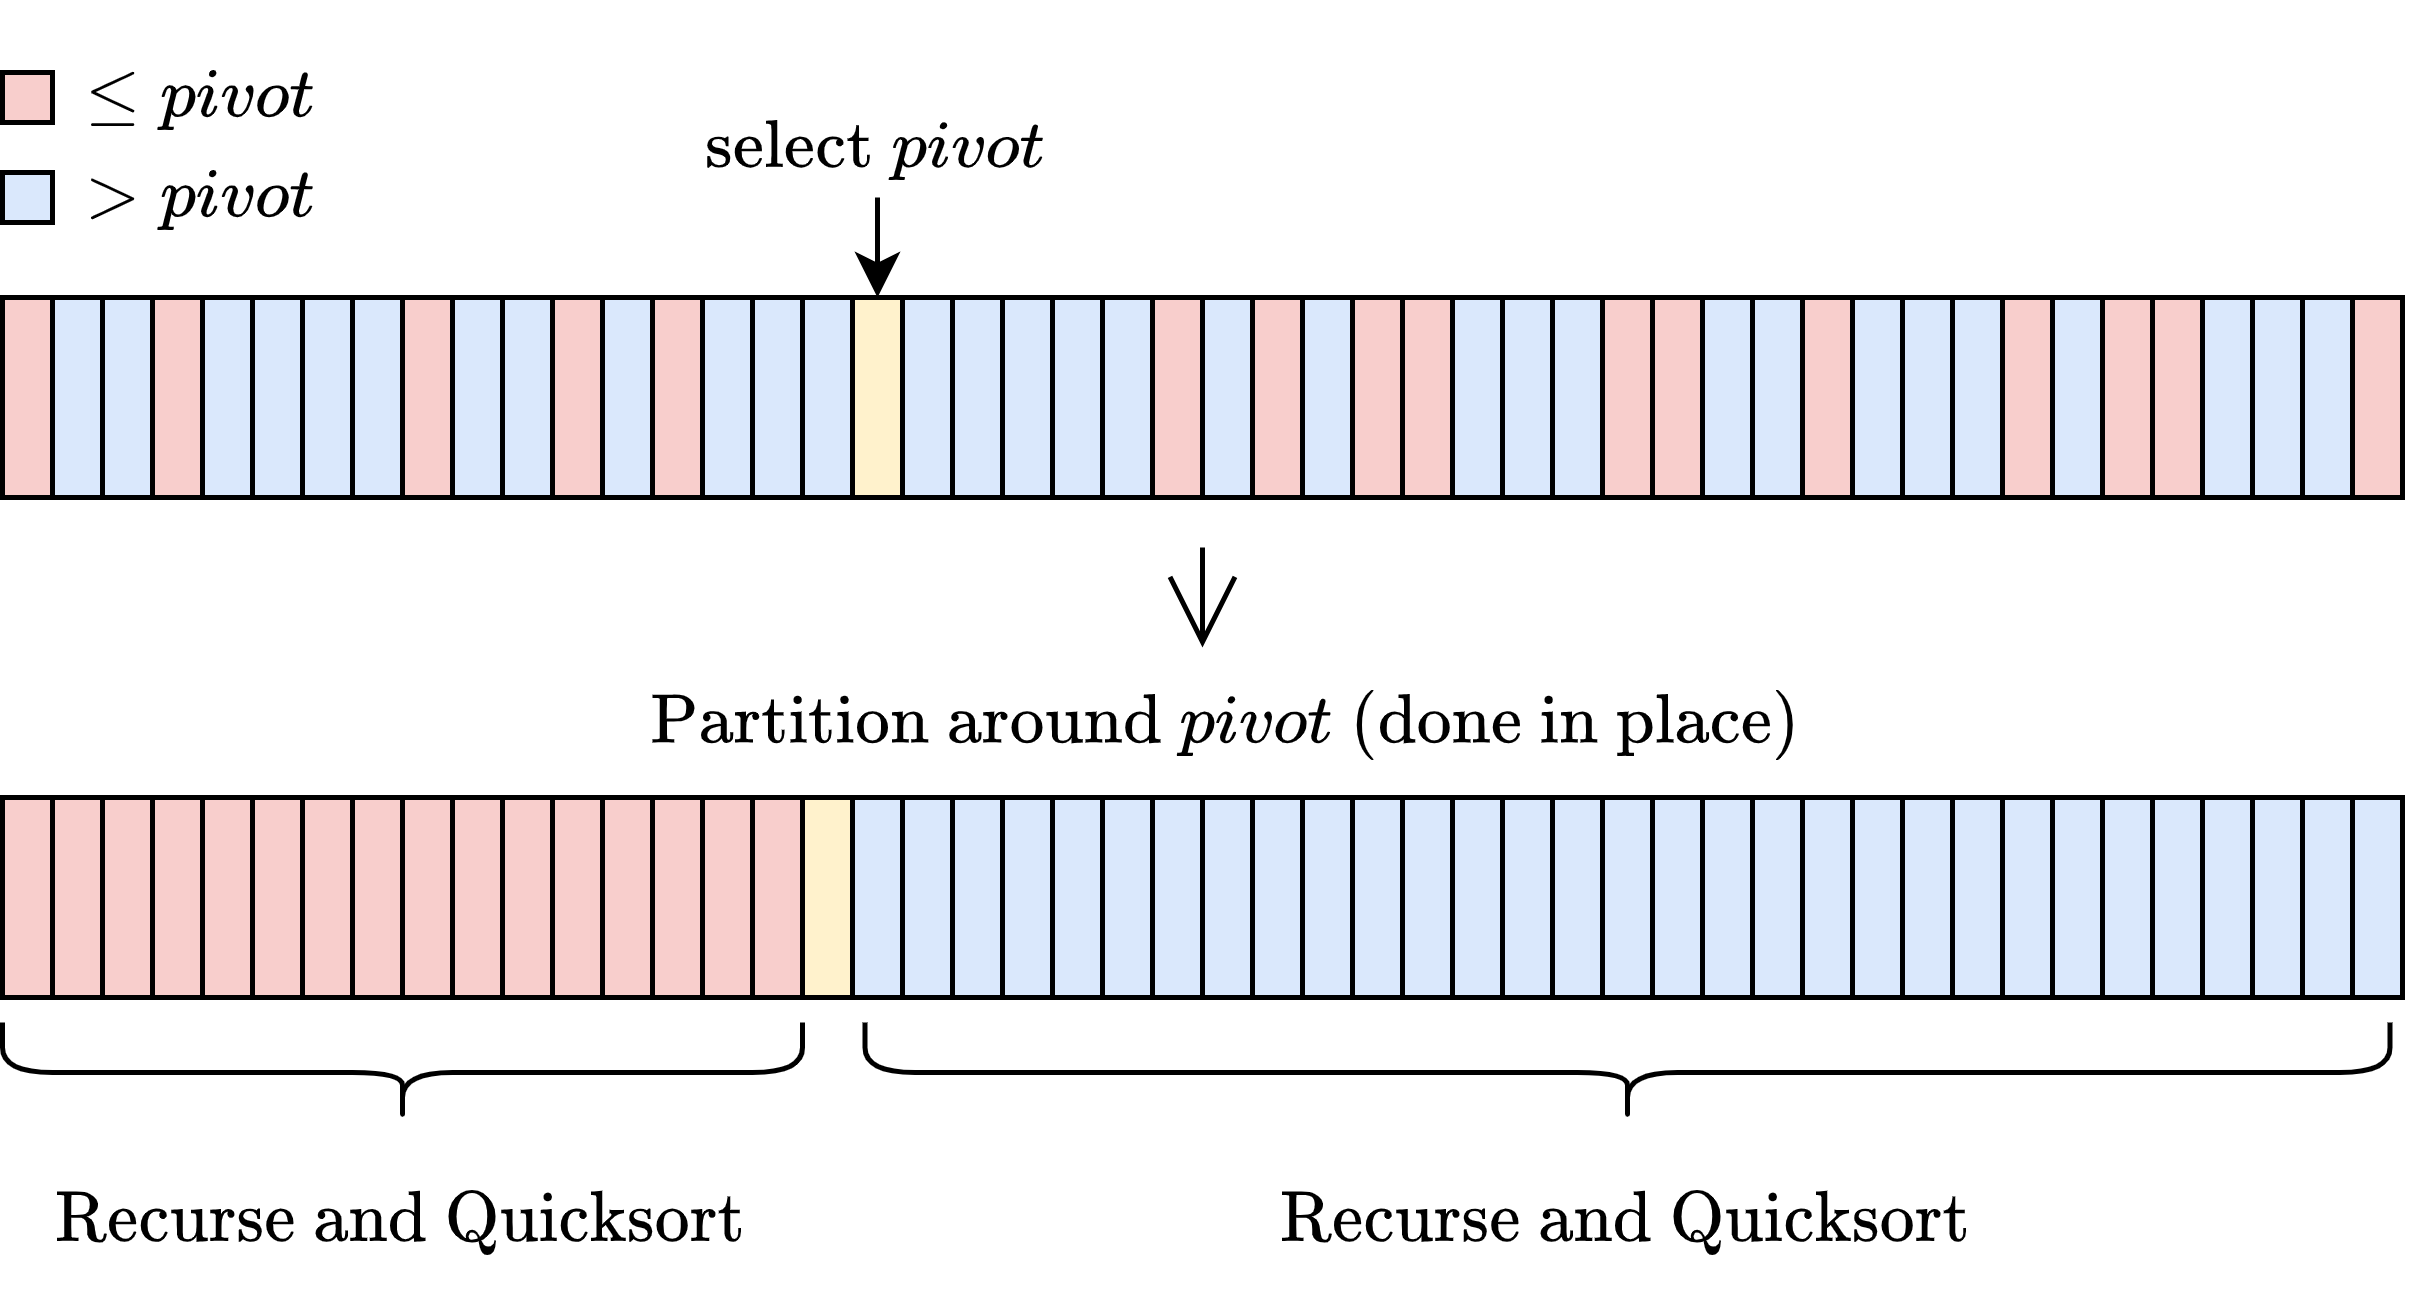
\includegraphics[width=.9\textwidth]{algorithms_and_indices/images/quicksort.drawio.png}
\end{center}
\inputminted{cpp}{algorithms_and_indices/code/quicksort.cpp}
\begin{center}
    \begin{tabular}{c | c}
        \textbf{Average Complexity} & \textbf{Worst-Case Complexity} \\
        $O(n \log n)$ & $O(n^2)$ \\ 
    \end{tabular}
\end{center}
Selecting a balanced pivot (ideally the median) is important to avoid worst-case complexity (where all others are larger or smaller than the pivot). Sampling multiple possible pivots negates this, as do other hybrid sorts.

\begin{tabbox}{prosbox}
    \textbf{Quick} & On average typically faster than merge or heapsort. \\
    \textbf{In-Place} & Sort can be performed entirely in place (no extra memory required, good temporal locality). \\
    \textbf{Parallel} & Is trivial to parallelise. \\
\end{tabbox}
\begin{tabbox}{consbox}
    \textbf{Worst-Case} & Avoiding $O(N^2)$ \\
    \textbf{Blind} & Does not take advantage of partially sorted data (in fact this can lead to worst-case depending on pivot selection). \\
\end{tabbox}

\begin{sidenotebox}{Better quicksorts}
    Many variations have been developed to improve performance, such as: 
    \\\begin{tabular}{l p{.7\textwidth}}
        \textit{Multi-Pivot Quicksort}       & For improved cache performance (a dual-pivot quicksort was used in Java 7). \\
        \textit{Quick-Radix Sort}            & Partitions based on bit (depth of recursion) of the key. \\
        \textit{Pattern Defeating Quicksort} & A hybrid sort using quicksort's fast average complexity, and heapsort's good worst-case complexity. \\
    \end{tabular}
\end{sidenotebox}
\subsection{Merge Sort}

\subsection{Tim Sort}

\subsection{Radix Sort}

\subsection{Top-N with Heaps}

\unfinished

\section{Joins}
\subsection{Database Normalisation (unassessed)}
% Normal Forms
\unfinished

\subsection{Join Types}
Normalised databases naturally require joins to re-compose data.

\begin{examplebox}{We would be honoured if you would join us\dots}
    Provide some examples of types of queries that would require a join.
    \tcblower
    \unfinished
\end{examplebox}

\begin{definitionbox}{Join}
    A join is a cross product with selection using data from both relations ($\sigma_{p(R_A.x, R_B.y)} (R_A \times R_B)$).
\end{definitionbox}

\subsubsection{Inner Joins}
\begin{tcbraster}[raster columns=2, raster equal height]
    \begin{definitionbox}{Inner Join}
        A join only returning rows from both tables which satisfy a predicate/condition.
        \begin{center}
            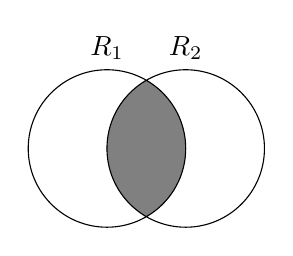
\begin{tikzpicture}[fill=gray]
                % left hand
                \scope
                \clip (1,0) circle (1);
                \fill (0,0) circle (1);
                \endscope
                % right hand
                \scope
                \clip (0,0) circle (1);
                \fill (1,0) circle (1);
                \endscope
                % outline
                \draw (0,0) circle (1) (0,1)  node [text=black,above] {$R_1$}
                      (1,0) circle (1) (1,1)  node [text=black,above] {$R_2$};
            \end{tikzpicture}
        \end{center}
    \end{definitionbox}
    \begin{definitionbox}{Natural Join}
        Joining two tables with an implicit join clause (join on equality on a column present in both tables
        \[R_1 \bowtie R_2\]
        \begin{minted}{sql}
FROM R1 NATURAL JOIN R2
FROM R1 JOIN R2 USING(id)
        \end{minted}
    \end{definitionbox}
\end{tcbraster}
\begin{tcbraster}[raster columns=2, raster equal height]
    \begin{definitionbox}{Theta Join}
        Joining two tables based on a condition/predicate $\theta$.
        \[R_1 \overset{\theta}{\bowtie} R_2\]
        \begin{minted}{sql}
FROM R1, R2 WHERE theta(R1, R2)
FROM R1 JOIN R2 ON theta(R1, R2)
        \end{minted}
    \end{definitionbox}
    \begin{definitionbox}{Equi Join}
        A \textbf{theta join} with a single equivalence condition. A \textbf{natural join} is an implicit \textbf{equi join}.
        \[R_1 \bowtie_{R_1.x = R_2.x}\]
        \begin{minted}{sql}
FROM R1, R2 WHERE R1.x = R2.x
        \end{minted}
    \end{definitionbox}
\end{tcbraster}
\begin{tcbraster}[raster columns=2, raster equal height]
    \begin{definitionbox}{Cross Join}
        Just cartesian product with no selection.
        \[R_1 \times R_2\]
        \begin{minted}{sql}
    FROM R1, R2
    FROM R1 CROSS JOIN R2
        \end{minted}
    \end{definitionbox}
    \begin{definitionbox}{Anti Join}
        A \textbf{theta join} using an inequality predicate
        \[R_1 \bowtie_{R_1.x <> R_2.x} R_2\]
        \begin{minted}{sql}
FROM R1 JOIN R2 ON R1.x <> R2.x
        \end{minted}
    \end{definitionbox}
\end{tcbraster}

\subsubsection{Outer Joins}
\begin{tcbraster}[raster columns=2, raster equal height]
    \begin{definitionbox}{Left Join}
        \[R_1 \overset{L}{\bowtie} R_2\]
        Returns all rows of $R_1$ even if no rows in $R_2$ match (in which case columns are \mintinline{sql}{NULL}).
        
            \begin{center}
                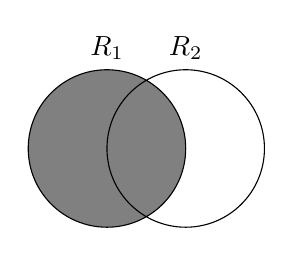
\begin{tikzpicture}[fill=gray]
                    % left hand
                    \scope
                    \fill (0,0) circle (1);
                    \endscope
                    % right hand
                    \scope
                    \clip (0,0) circle (1);
                    \fill (1,0) circle (1);
                    \endscope
                    % outline
                    \draw (0,0) circle (1) (0,1)  node [text=black,above] {$R_1$}
                            (1,0) circle (1) (1,1)  node [text=black,above] {$R_2$};
                \end{tikzpicture}
            \end{center}
            \begin{minted}{sql}
FROM R1 LEFT JOIN R2 ON ... 
            \end{minted}
    \end{definitionbox}
    \begin{definitionbox}{Right Join}
        \[R_1 \overset{R}{\bowtie} R_2\]
        Returns all rows of $R_2$ even if no rows in $R_1$ match (in which case columns are \mintinline{sql}{NULL}).
            \begin{center}
                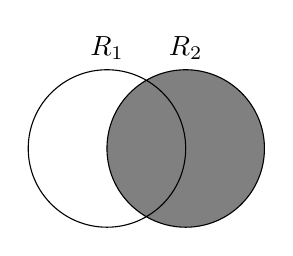
\begin{tikzpicture}[fill=gray]
                    % left hand
                    \scope
                    \clip (1,0) circle (1);
                    \fill (0,0) circle (1);
                    \endscope
                    % right hand
                    \scope
                    \fill (1,0) circle (1);
                    \endscope
                    % outline
                    \draw (0,0) circle (1) (0,1)  node [text=black,above] {$R_1$}
                            (1,0) circle (1) (1,1)  node [text=black,above] {$R_2$};
                \end{tikzpicture}
            \end{center}
            \begin{minted}{sql}
FROM R1 RIGHT JOIN R2 ON ... 
            \end{minted}
    \end{definitionbox}
\end{tcbraster}
\begin{definitionbox}{Full Outer Join}
    \[R_1 \overset{O}{\bowtie} R_2 \equiv R_1 \overset{L}{\bowtie} R_2 \cup R_1 \overset{R}{\bowtie} R_2\]
    Returns all rows from all tables matching, with rows from either $R_1$ or $R_2$ that do not have match associated with \mintinline{sql}{NULL} columns from the other table.
    \begin{center}
        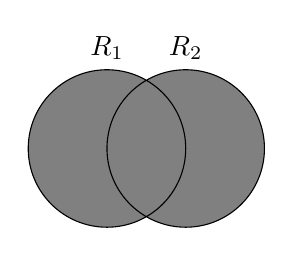
\begin{tikzpicture}[fill=gray]
            % left hand
            \scope
            \fill (0,0) circle (1);
            \endscope
            % right hand
            \scope
            \fill (1,0) circle (1);
            \endscope
            % outline
            \draw (0,0) circle (1) (0,1)  node [text=black,above] {$R_1$}
                    (1,0) circle (1) (1,1)  node [text=black,above] {$R_2$};
        \end{tikzpicture}
    \end{center}
    \begin{minted}{sql}
FROM R1 FULL OUTER JOIN R2 ON ... 
FROM R1 FULL JOIN R2 ON ... 
FROM (SELECT * FROM R1 LEFT JOIN R2 ON ... UNION SELECT * FROM R1 RIGHT JOIN R2 ON ...)
    \end{minted}
\end{definitionbox}


\begin{examplebox}{Which imposter?}
    Which of the following are joins?
    \begin{multicols}{2}
    \begin{enumerate}
        \item {
\begin{minted}{sql}
SELECT R.r, S.s
FROM R, S
WHERE R.id = S.id;
\end{minted}
}
\item {
    \begin{minted}{sql}
SELECT R.r, S.s
FROM R, S
WHERE R.r = R.id
    \end{minted}
}
        \item {
        \begin{minted}{sql}
SELECT R.r
FROM R, S
WHERE R.id = S.id;
        \end{minted}
        }
        \item {
            \begin{minted}{sql}
SELECT R.r
FROM R, S
WHERE R.r = "some string";
            \end{minted}
        }
    \end{enumerate}
    \end{multicols}
    \tcblower
    \begin{enumerate}
        \item \textbf{Join} (Selects on both $R$ and $S$)
        \item \textbf{Not a Join} (Only selects on $R$)
        \item \textbf{Join} (The $\sigma$ selection is on $R$ and $S$, so a join even if only $R$ is projected)
        \item \textbf{Not a Join} (Only selects on $R$)
    \end{enumerate}
\end{examplebox}

\subsection{Join Implementations}
The following join implementations are written is C++20
\begin{minted}{cpp}
#include <algorithm>
#include <iostream>
#include <tuple>
#include <unordered_map> // using contains from cpp20
#include <utility>
#include <vector>

using namespace std;

template <typename... types> using Table = vector<tuple<types...>>;
\end{minted} 
Compile with \mintinline{bash}{g++ -std=c++2a joins.cc}, the following main can be used for testing:
\begin{minted}{cpp}
int main() {
  vector<tuple<int, char, int>> table1{
      {1, 'a', 21}, {1, 'b', 34}, {2, 'c', 23}};
  vector<tuple<char, int>> table2{{'a', 21}, {'b', 34}, {'c', 6}};

  auto tableResult = sort_merge_join<2, 1>(table1, table2);

  print_table(table1);
  print_table(table2);
  print_table(tableResult);
}
\end{minted}
\mintinline{cpp}{#include "print_table.cc"} after the \mintinline{cpp}{using Table = ...} definition for easy printing.

\subsection{Nested Loop Join}
We can implement a basic join naively using nested loops.
\begin{minted}{Cpp}
template <size_t leftCol, size_t rightCol, typename... TypesOne, typename... TypesTwo>
Table<TypesOne..., TypesTwo...> nest_loop_join(Table<TypesOne...> &left, Table<TypesTwo...> &right) {
  Table<TypesOne..., TypesTwo...> result;
  for (auto &leftElem : left) for (auto &rightElem : right) {
    if (get<leftCol>(leftElem) == get<rightCol>(rightElem)) {
      result.push_back(tuple_cat(leftElem, rightElem));
    }
  }
  return result;
}
\end{minted}
\[\text{Time Complexity} = \begin{cases}
    \cfrac{\Theta (|left| \times |right|) }{2} & \text{ If elements unique} \\
    \Theta (|left| \times |right|)  & otherwise \\
\end{cases}\]
\begin{tabbox}{prosbox}
    \textbf{Simple} & Easy to reason about (memory accesses \& complexity) \\
    \textbf{Trivially Parallel} & Loop iterations are not dependent, so can be parallelised. \\
    \textbf{Sequential I/O} & Access is done in the order of the tables storage (sequential access better for both memory \& disk) \\
\end{tabbox}
\begin{tabbox}{consbox}
    \textbf{Performance} & Linear time complexity. \\
\end{tabbox}

\subsection{Sort Merge Join}
If we assume both tables are sorted, and values (being joined on) are unique.
\begin{itemize}
  \item Two cursors (one per table)
  \item Advance cursors in order, if the value on the left exceeds the right there can be no joins for the left row (and vice versa).
\end{itemize}
\begin{minted}{cpp}
template <size_t leftCol, size_t rightCol, typename... TypesOne,
          typename... TypesTwo>
Table<TypesOne..., TypesTwo...> sort_merge_join(const Table<TypesOne...> &leftT,
                                                const Table<TypesTwo...> &rightT) {

  Table<TypesOne..., TypesTwo...> result;

  // copy tables and sort (required for interface, but could be ommitted with assumption)
  auto left = leftT;
  auto right = rightT;
  sort(left.begin(), left.end(), [](auto const &a, auto const &b) {
    return get<leftCol>(a) < get<leftCol>(b);
  });
  sort(right.begin(), right.end(), [](auto const &a, auto const &b) {
    return get<rightCol>(a) < get<rightCol>(b);
  });

  auto leftIndex = 0;
  auto rightIndex = 0;

  while (leftIndex < left.size() && rightIndex < right.size()) {
    auto leftElem = left[leftIndex];
    auto rightElem = right[rightIndex];

    if (get<leftCol>(leftElem) < get<rightCol>(rightElem)) {
      leftIndex++;
    } else if (get<leftCol>(leftElem) > get<rightCol>(rightElem)) {
      rightIndex++;
    } else {
      result.emplace_back(tuple_cat(leftElem, rightElem));
      leftIndex++;
      rightIndex++;
    }
  }

  return result;
}
\end{minted}
\[\begin{split}
  \text{Time Complexity} &= \Theta (sort(left)) + \Theta (sort(right)) + \Theta (merge) \\
  & = \Theta(|left| \times \log |left| + |right| \times \log |right| + |left| + |right|)
\end{split}\]
\begin{tabbox}{prosbox}
  \textbf{Sequential I/O} & In the merge phase \\
  \textbf{Inequality} & Works for joins using $<$ and $>$ instead of just \textit{equi-joins}. \\
\end{tabbox}
\begin{tabbox}{consbox}
  \textbf{Tricky to Parallelize} & Sorts can be somewhat parallelised, but merge is sequential. \\
\end{tabbox}

\subsection{Hash Join}
For \textit{equi joins} we can insert one table into a hash table, then iterate over the second (assumed constant time lookup in hashtable).
\\
\\ Below we have used the standard template library's \mintinline{cpp}{unordered_map} 
\begin{minted}{cpp}
template <size_t leftCol, size_t rightCol, typename... TypesOne, typename... TypesTwo>
Table<TypesOne..., TypesTwo...> hash_join(const Table<TypesOne...> &left,
                                          const Table<TypesTwo...> &right) {
  Table<TypesOne..., TypesTwo...> result;
  using leftColType = typename tuple_element<leftCol, tuple<TypesOne...>>::type;
  
  // Build Phase - create has hashtable of one table.
  // we should ideally choose the smallest table here -> smallest hashmap
  unordered_map<leftColType, const tuple<TypesOne...> *> leftContents(
      left.size());

  // Inserting pointers to avoid overhead of cloning tuples
  for (const tuple<TypesOne...> &elem : left) {
    leftContents.insert(make_pair(get<leftCol>(elem), &elem));
  }

  // Probing phase - find matching values
  for (auto &elem : right) {
    if (leftContents.contains(get<rightCol>(elem))) {
      result.emplace_back(tuple_cat(*leftContents[get<rightCol>(elem)], elem));
    }
  }

  return result;
}
\end{minted}
\[\begin{split}
    \Theta (|build| + |probe|) & \text{best case} \\
    O(|build| \times |probe|) & \text{worst case} \\
\end{split}\]
\begin{itemize}
    \item The probing phase can be easily parallelised (hashtable is unchanged), however the build side is tricky to paralleliuse efficiently.
\end{itemize}
\begin{tabbox}{prosbox}
    \textbf{Time Complexity} & (Assuming the lookup is constant time). \\
    \textbf{Hashing} & Need to avoid collisions, keep time calculating hash low, and be applicable to many data types. \\
\end{tabbox}
\begin{tabbox}[.7\textwidth]{consbox}
    \textbf{Space Complexity} & Requires building a hashtable structure (assumning the table was not stored as this already). Best when one relation is much smaller than the other (use smallest). \\
    \textbf{Expensive Hashing} & Some good hashing algorithms are expensive (potentially as many cycles as multiple data accesses). \\
\end{tabbox}

\begin{sidenotebox}{Bucket Based Hashmaps}
    Many hashmaps are implemented as a table of buckets (linked lists of conflicting values). 
    \begin{itemize}
        \item Called bucket-chaining/open addressing
        \item Poor lookup performance.
        \item Good insert performance (can prepend to bucket linked list on conflict).
    \end{itemize}
\end{sidenotebox}


\section{Hash Tables}
\subsection{Probing Hashmap}
\begin{center}
    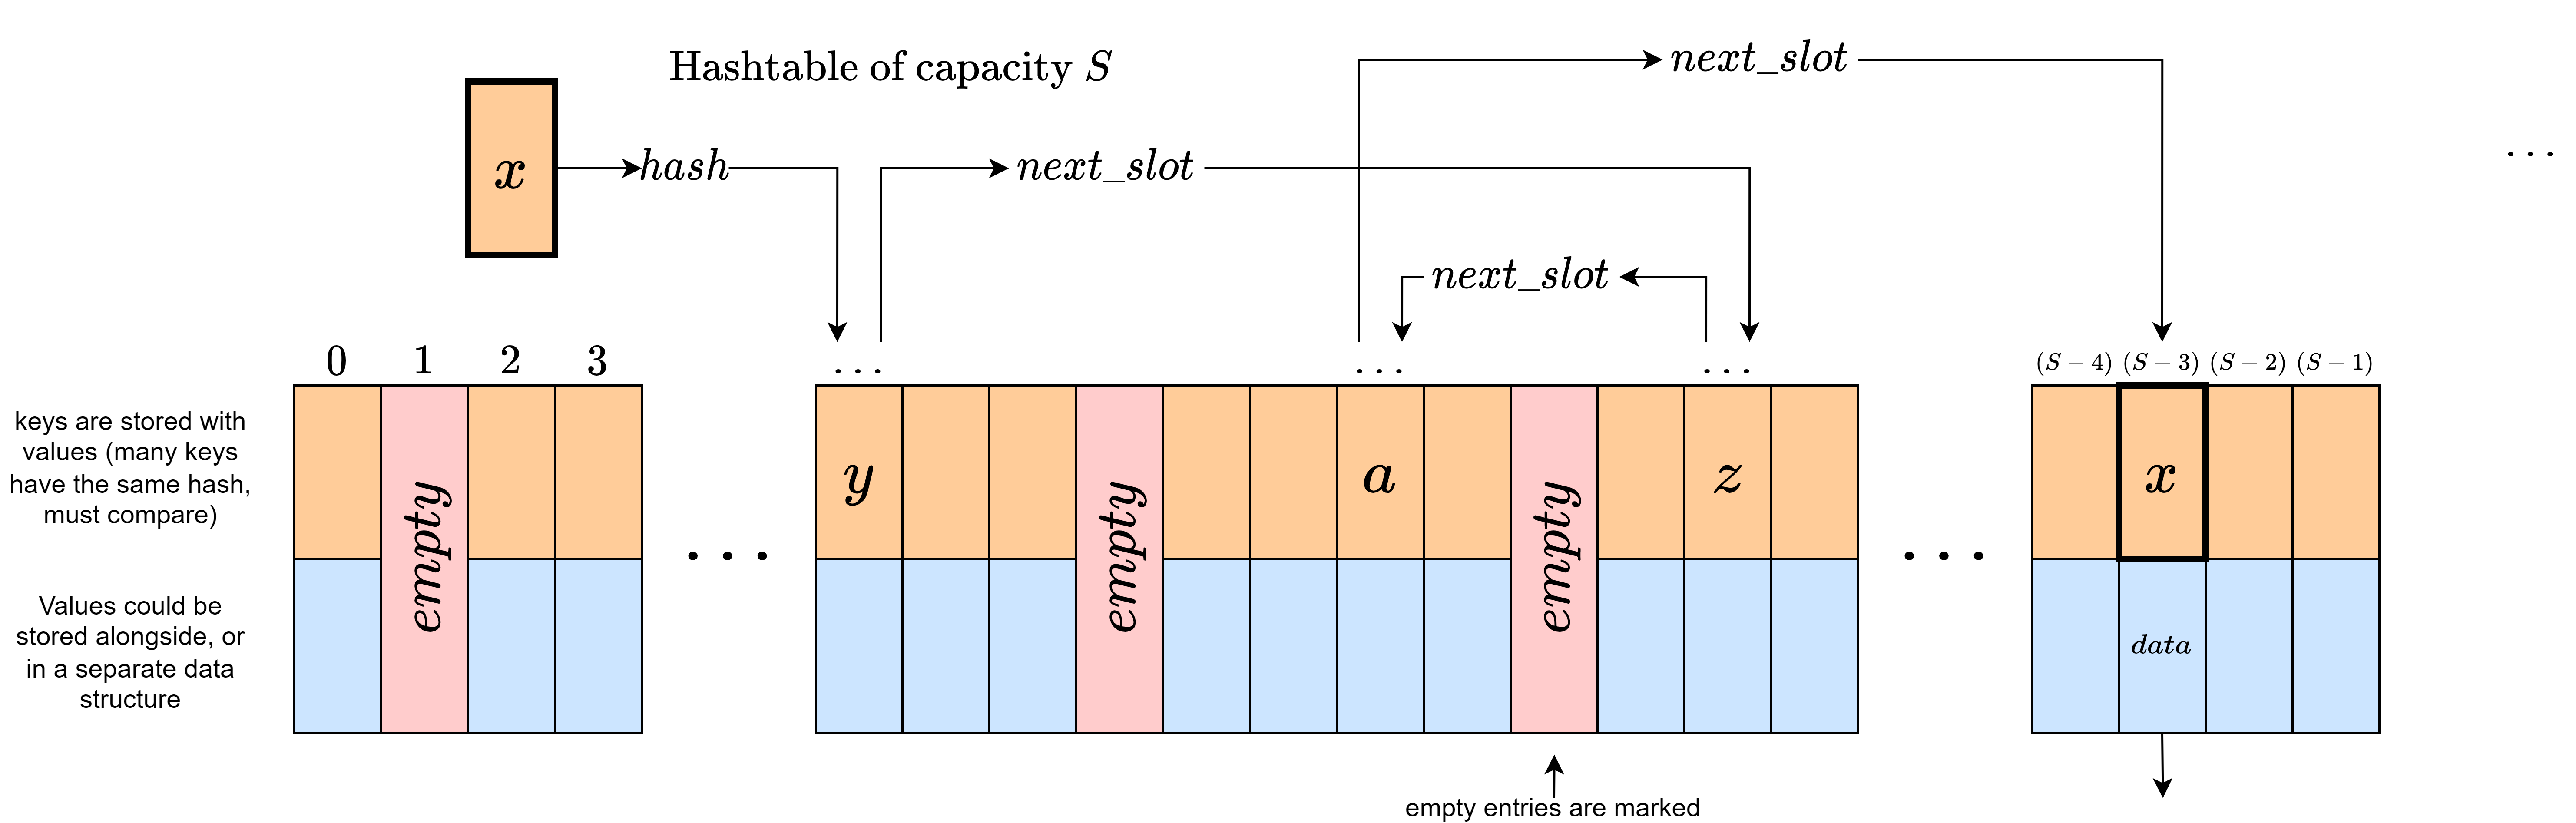
\includegraphics[width=.9\textwidth]{algorithms_and_indices/images/hash_table.drawio.png}
\end{center}
We can define the hash function using a \mintinline{cpp}{struct} as follows:
\begin{minted}{cpp}
template <typename T> struct Probe {
  virtual void hash(T data, size_t indexSize) = 0;
  virtual size_t next() = 0;
};
\end{minted}
\begin{center}
    \begin{tabular}{l l p{.6\textwidth}}
        Requirement & \textbf{Pure} & no state/call with same value $\to$ same hash \\
        Requirement & \textbf{Known Co-Domain} & Known range of values (co-domain also known as image/range). \\
        Nicety & \textbf{Contiguous Co-Domain} & No gaps in range of output means few gaps holes in the table. \\
        Nicety & \textbf{Uniform} & All hash values in the range are equally likely. \\
    \end{tabular}
\end{center}
\begin{sidenotebox}{Typical Hashers}
    \begin{center}
        \begin{tabular}{l p{.8\textwidth}}
            \textbf{MD5} & Encodes any length string as a 128-bit hash. \\
            \textbf{Modulo-Division} & Very simple and fast. \\
            \textbf{MurmurHash} & A fast, non-cryptographic hash (\href{https://github.com/aappleby/smhasher}{on github}). \\
            \textbf{CRC32} & Cyclic Redundancy Check (common, non-cryptographic) and with hardware support on some systems (also see usage of \mintinline{asm}{PCLMULQDQ} on intel for acceleration \href{https://www.intel.com/content/dam/www/public/us/en/documents/white-papers/fast-crc-computation-generic-polynomials-pclmulqdq-paper.pdf}{here})
        \end{tabular}
    \end{center}
\end{sidenotebox}
\begin{examplebox}{Hash it out}
    Write a basic Modulo-Division hash using the interface above provided. Take the modulus as a template parameter.
    \tcblower
    \begin{minted}{cpp}
template <size_t MODULUS> size_t modulusHash(int data) {
  return static_cast<size_t>(data) % MODULUS;
}
    \end{minted}
\end{examplebox}
When different keys have the same hash a \textit{conflict} occurs. A strategy is required to select the next slot to probe (the \mintinline{cpp}{nextSlot} function).
\begin{itemize}
    \item We want locality (when detecting a conflict, the real key is close/same page/line)
    \item Very high locality will result in parts of the hash table being saturated, and long probe chains.
    \item We want to avoid leaving holes (may be used by hash function, but if the probing function never accesses, they are likely to never be used)
\end{itemize}

\subsubsection{Linear Probing}
Add some \mintinline{cpp}{DISTANCE} to the probe position, wrap around at the end of the buffer.
\begin{minted}{cpp}
template <typename K> struct LinearProbe : public Probe<K> {
  LinearProbe(std::function<size_t(K)> hash) : _hash(hash) {}

  void hash(K data, size_t indexSize) override {
    _indexSize = indexSize;
    _position = _hash(data) % indexSize;
  };

  size_t next() override {
    auto oldPosition = _position;
    _position = (_position + 1) % _indexSize;
    return oldPosition;
  };

private:
  std::function<size_t(K)> _hash;
  size_t _position;
  size_t _indexSize;
};
\end{minted}
\begin{tabbox}{prosbox}
    \textbf{Simple} & Easy to reason about memory access pattern. \\
    \textbf{Locality} & Can alter \mintinline{cpp}{DISTANCE} to place values as \textit{adjacently} as we need. \\
\end{tabbox}
\begin{tabbox}[.7\textwidth]{consbox}
    \textbf{Long Probe-Chains} & From too much locality on adversarial input data (can input data to the table to create worse case conflicts (and hence probe chain length) scenario) \\
\end{tabbox}

\subsubsection{Quadratic Probing}
\[P, P + 1^2, P + 2^2, P + 3^2, \dots, P + n^2, \dots\]
\begin{itemize}
    \item Wrap around end of table.
    \item Variants exist (still use power of $2$ but can include linear and constant term)
\end{itemize}
\begin{minted}{cpp}
template <typename K> struct QuadraticProbe : public Probe<K> {
  QuadraticProbe(std::function<size_t(K)> hash) : _hash(hash) {}

  void hash(K data, size_t indexSize) override {
    _indexSize = indexSize;
    _firstPosition = _hash(data) % indexSize;
    _step = 0;
  };

  size_t next() override {
    auto newPosition = _firstPosition + _step * _step;
    _step++;
    return newPosition;
  };

private:
  std::function<size_t(K)> _hash;
  size_t _firstPosition;
  size_t _step;
  size_t _indexSize;
};
\end{minted}
\begin{tabbox}{prosbox}
    \textbf{Simple} & Easy to reason about memory access pattern. \\
    \textbf{Locality} & for first probes is good. \\
\end{tabbox}
\begin{tabbox}{consbox}
    \textbf{Conflicts} & Experiences conflicts in first probes where is it similar to linear. \\
\end{tabbox}

\subsubsection{Rehashing}
In order to distribute nodes uniformly, use a has function to hash a conflicting position to find the next one.
\begin{minted}{cpp}
template <typename K> struct ReHashProbe : public Probe<K> {
  ReHashProbe(std::function<size_t(K)> hash,
              std::function<size_t(size_t)> rehash)
      : _hash(hash), _rehash(rehash) {}

  void hash(K data, size_t indexSize) override {
    _indexSize = indexSize;
    _current = _hash(data) % indexSize;
  };

  size_t next() override {
    auto old = _current;
    _current = _rehash(_current) % _indexSize;
    cout << "rehashing to " << _current << endl;
    return old;
  };

private:
  std::function<size_t(K)> _hash;
  std::function<size_t(size_t)> _rehash;
  size_t _current;
  size_t _indexSize;
};
\end{minted}
\begin{tabbox}{prosbox}
    \textbf{Simple} & To implement \\
    \textbf{Reuse} & Can potentially reuse the hashing function. \\
\end{tabbox}
\begin{tabbox}{consbox}
    \textbf{Locality} & is poor as probes distributed uniformly. \\
    \textbf{Conflict Probability} & is constant (every probe may conflict with another element). \\
\end{tabbox}

\subsubsection{Resizing}
For the example above we have considered fixed-size hashmaps. 
\begin{itemize}
    \item Hashtables are typically overallocated by factor $2$ (twice as many slots as expected input tuples).
    \item Table can be resized once it is larger than some capacity (will change hash of values, so must effectively rebuild hashmap)
    \item When determining cost we amortise (spread cost of resize over all inserts \& (for this module) assume this cost is constant per insert).
\end{itemize}
For this reason, hash-joins (using hash tables) are best when one of the joined relations is much smaller than the other.

\subsubsection{Deleting with Markers}
\begin{center}
    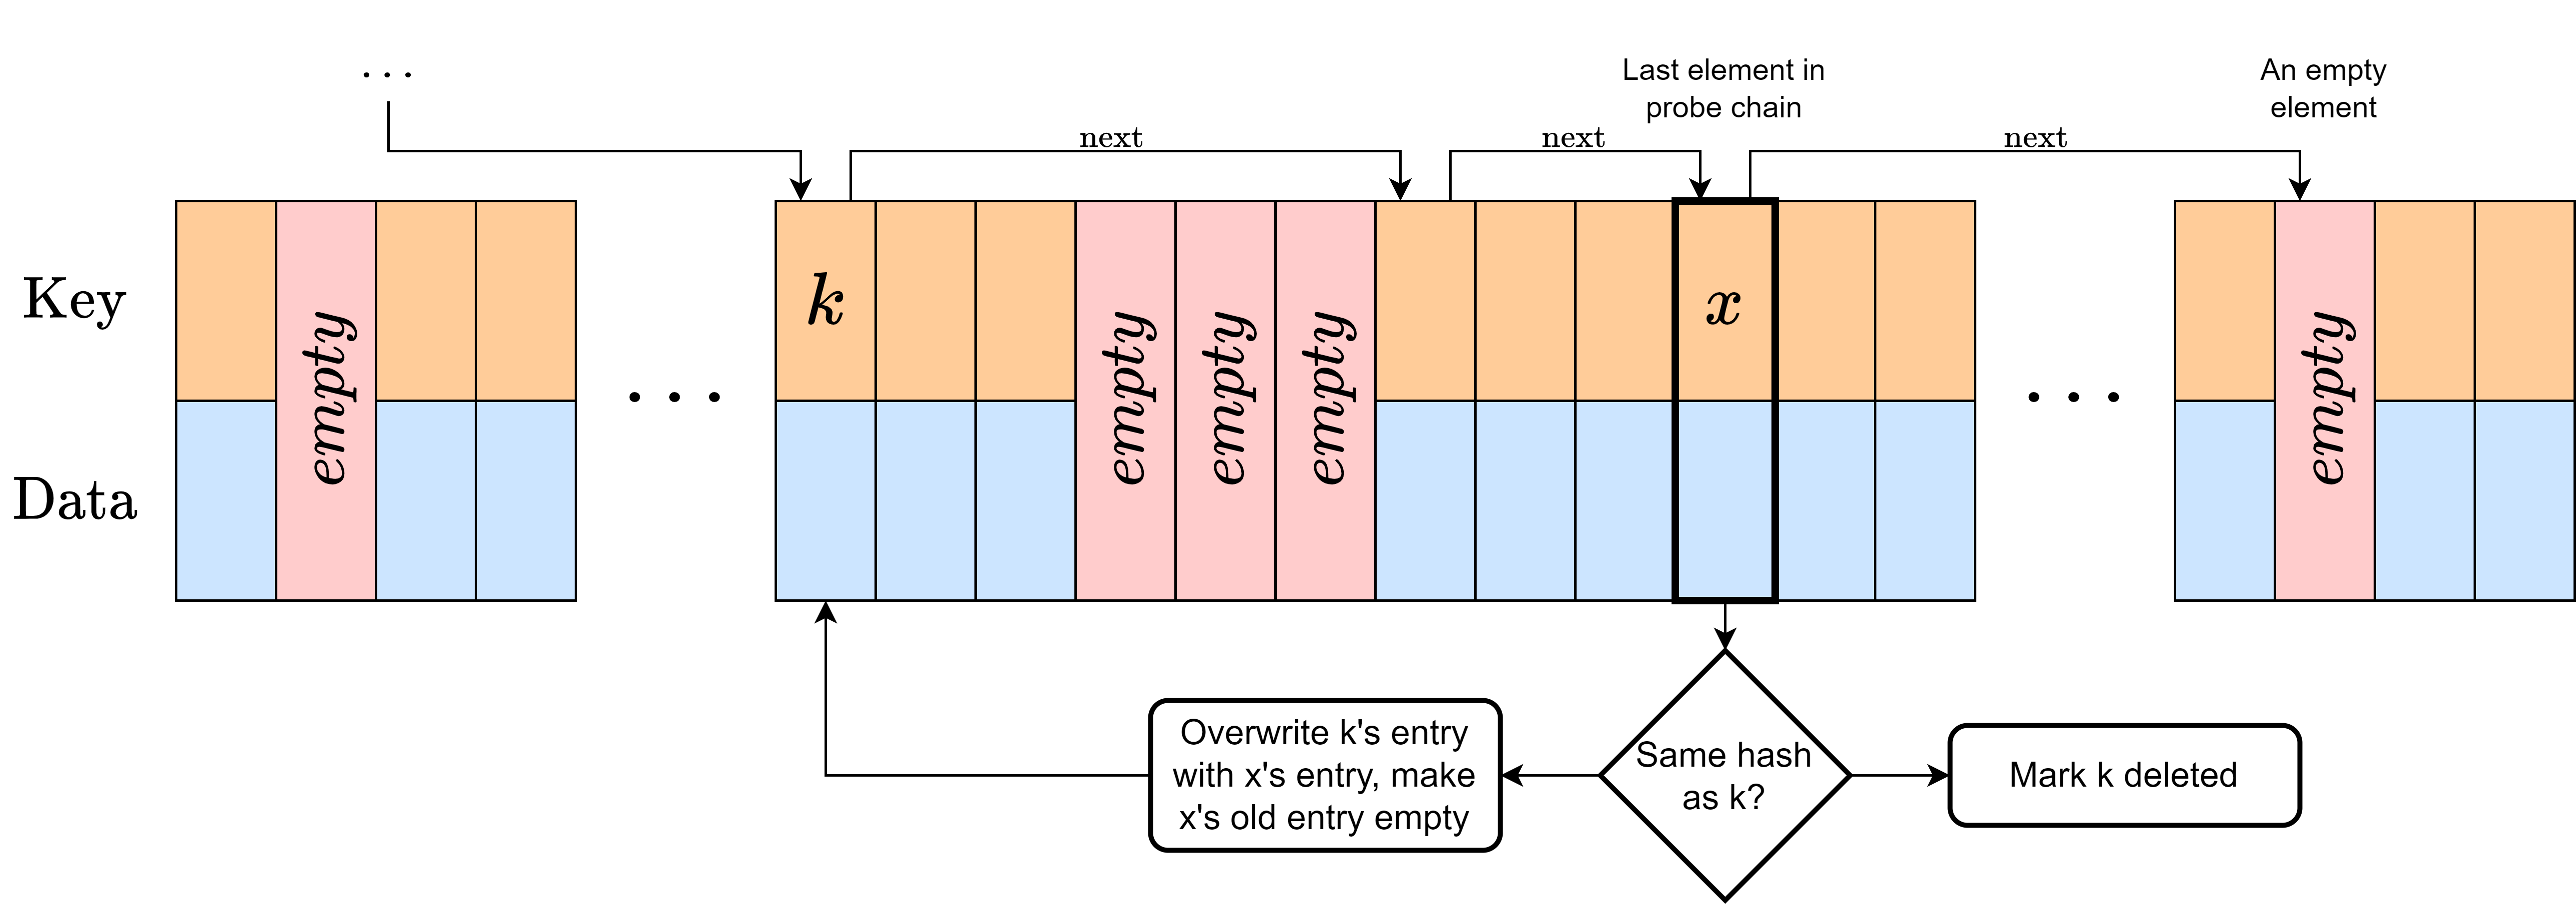
\includegraphics[width=.8\textwidth]{algorithms_and_indices/images/mark_deletion.drawio.png}
\end{center}
An implementation is included below:
\subsection{Basic Hash Table Implementation}
\begin{sidenotebox}{Contribute!}
    This basic implementation can be improved!
    \begin{itemize}
        \item Resize functionality
        \item Use structs for entries, rather than tuples
        \item Construct probers local to methods
        \item Provide prober type in template and construct, rather than taking constructor parameter
    \end{itemize}
\end{sidenotebox}

\inputminted{cpp}{algorithms_and_indices/code/hashtable.cc}

\subsection{Partitioning}
Sequential accesses are cheaper than random accesses, as they can access the same page in memory \& thus share the cost of the initially expensive cold access.
\[\begin{split}
    c &= \text{cost of page-in } \\
    \cfrac{n}{pagesize_{OS}} \times c  &= \text{cost of sequentially accessing }n \text{ elements}\\
    \cfrac{c}{pagesize_{OS}} &= \text{cost of one access} \\
\end{split}\]
In order to reduce the cost of accessing some data we can:
\begin{itemize}
    \item Increase the page size (huge pages).
    \item Make the access pattern \textit{more} sequential.
\end{itemize}
Assuming a hashtable does not fit in memory/buffer page cache, we can reduce costs from page-misses by paying less for a partitioning pass.

\unfinished

\subsection{Indexing}
We can use a secondary store of redundant data to speed up queries.
\begin{itemize}
    \item Denormalised (redundant) data is controlled by the DBMS.
    \item Can be created or removed without affecting the system (other than performance \& storage space).
    \item Semantically invisible to the user (cannot change semantics of queries).
    \item Can be used to speed up data access of some queries (e.g avoiding having to build a hashtable in hash join as it is already available).
    \item Occupy potentially considerable space.
    \item Must be maintained under updates.
    \item Must be considered by query optimiser.
\end{itemize}
\begin{definitionbox}{Clustered/Primary Index}
    An index storing all tuples of a table.
    \begin{itemize}
        \item Only one per table
        \item Can use more space than the table being indexed
        \item No redundant data / no duplicates within the index (only one copy for each tuple is indexed) (no consistency issues)
    \end{itemize}
\end{definitionbox}
\begin{definitionbox}{Unclustered/Secondary Index}
    Used to store pointers to tuples of a table.
    \begin{itemize}
        \item No limit on number of indexes
        \item Does not replicate data (the tuples pointed to in the table), but may replicate pointers (multiple pointers in index to the same tuple in the table) (some consistency issues)
    \end{itemize}
\end{definitionbox}
\subsubsection{SQL Indexes}
ANSI SQL supports the creation \& destruction of indexes by the user.
\begin{minted}{sql}
CREATE INDEX index_name ON table_name (column_1, column2, ...);
DROP INDEX index_name;
\end{minted}
\begin{itemize}
    \item Unclear what type of index is created
    \item No control over parameters (e.g hash table size)
\end{itemize}
The standard has been extended by SQL implementations to allow for finer control.
\begin{sidenotebox}{The elephant in the room}
    Among other DBMS, Postgres supports many types of index (\href{https://www.postgresql.org/docs/current/indexes.html}{documentation here})
    \begin{minted}{psql}
/* By default CREATE INDEX uses a B-Tree */
CREATE INDEX name ON table USING HASH (column);

/* It is even possible to only index certain parts of a table using a WHERE clause */
CREATE INDEX access_log_client_ip_ix ON access_log (client_ip)
WHERE NOT (client_ip > inet '192.168.100.0' AND
           client_ip < inet '192.168.100.255');
    \end{minted}
\end{sidenotebox}

\subsection{Hash Indexes}
An index backed by a hash table.
\begin{center}
    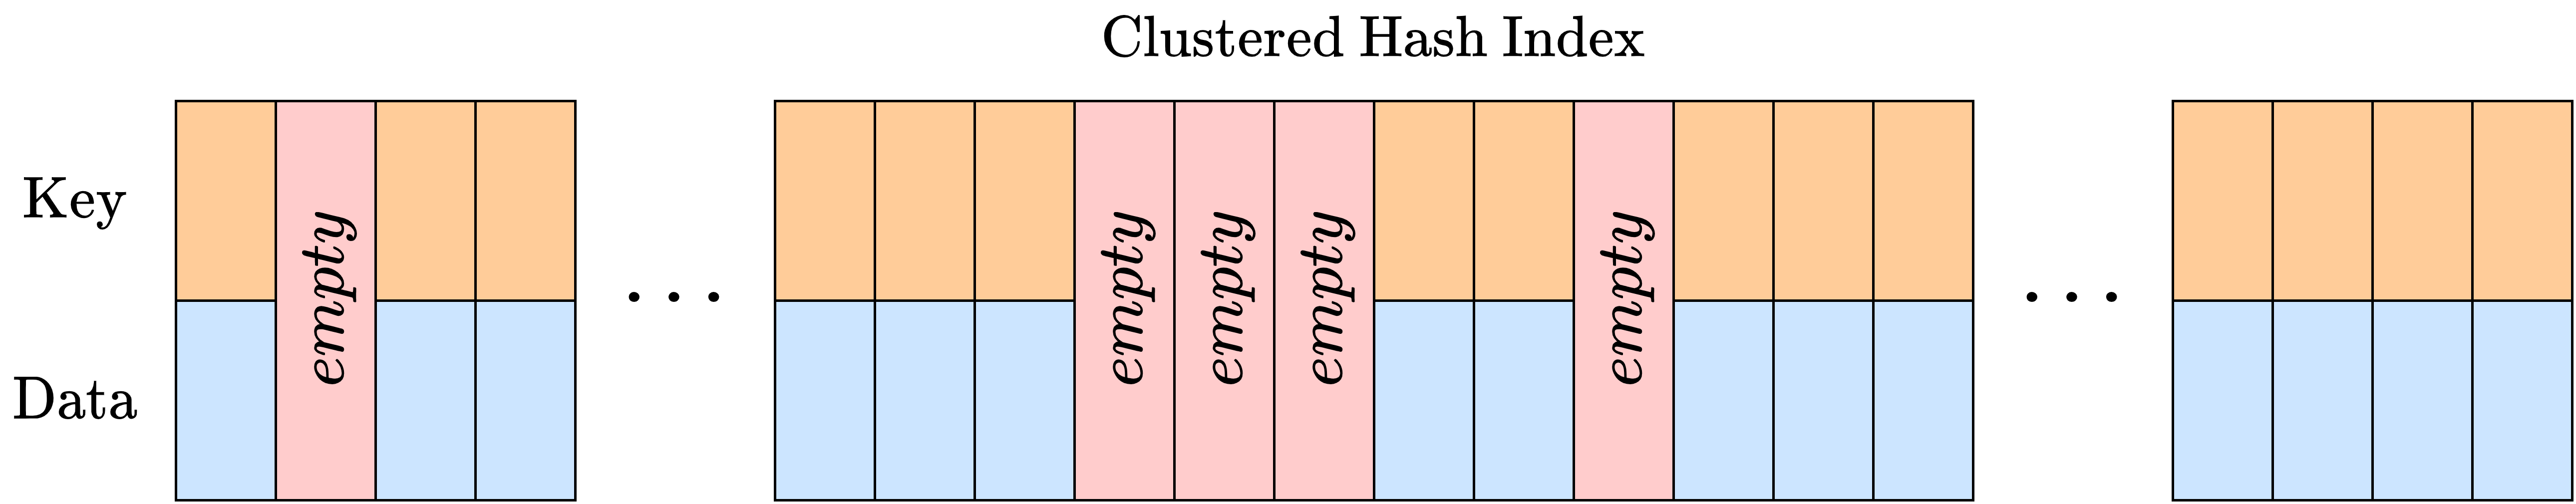
\includegraphics[width=.8\textwidth]{algorithms_and_indices/images/hash_index_clustered.drawio.png}
\end{center}
\begin{center}
    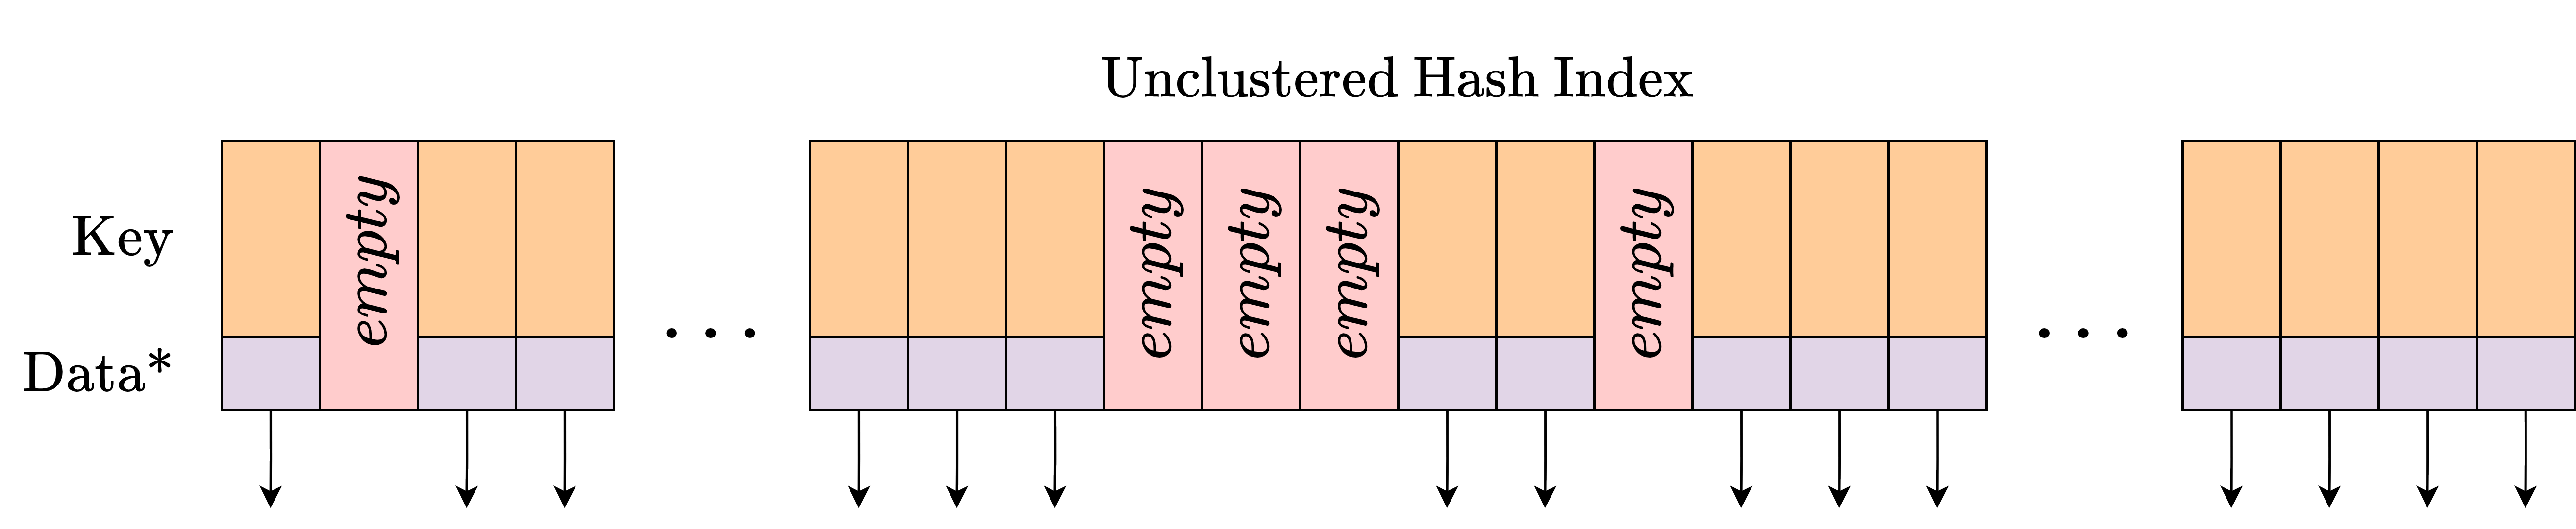
\includegraphics[width=.8\textwidth]{algorithms_and_indices/images/hash_index_unclustered.drawio.png}
\end{center}
Persistent hash tables may grow very large (overallocate) and need to be rebuilt to grow (can cause unexpected spike when an insert causes a rebuild).
\\
\\ Aside from the normal pros/cons of hash tables in general:
\begin{tabbox}[.7\textwidth]{prosbox}
    \textbf{Hash-Joins \& Aggregation} & Perform well and remove build phase (provided they index on the columns joining). \\
    \textbf{Equality Selection} & {Can reduce number of candidate columns if not all columns are indexed
    \begin{minted}{sql}
SELECT * FROM table_name WHERE column1 = some_value;
    \end{minted}
    } \\
\end{tabbox}

\begin{tabbox}{consbox}
    \textbf{Limited Applicability} & Not useful for queries not using equality. \\
\end{tabbox}

\subsection{Bitmap Indexing}
\begin{definitionbox}{Bit Vector}
    A sequence of 1 bit boolean values indicating some condition holds for indexes of another sequence.
    \[BV_{==3}([1,2,5,6,3,2,3,4]) = [0,0,0,0,1,0,1,0] \]
    \begin{itemize}
        \item Memory is byte addressable, and registers typically word-size (usually 32/64 bits).
        \item Some useful instructions (and compiler intrinsics) can be used.
        \item Can use SIMD instructions to operate on sections of a bitvector in parallel without using multithreading.
    \end{itemize}
\end{definitionbox}

\begin{definitionbox}{Bitmap Index}
    \begin{center}
        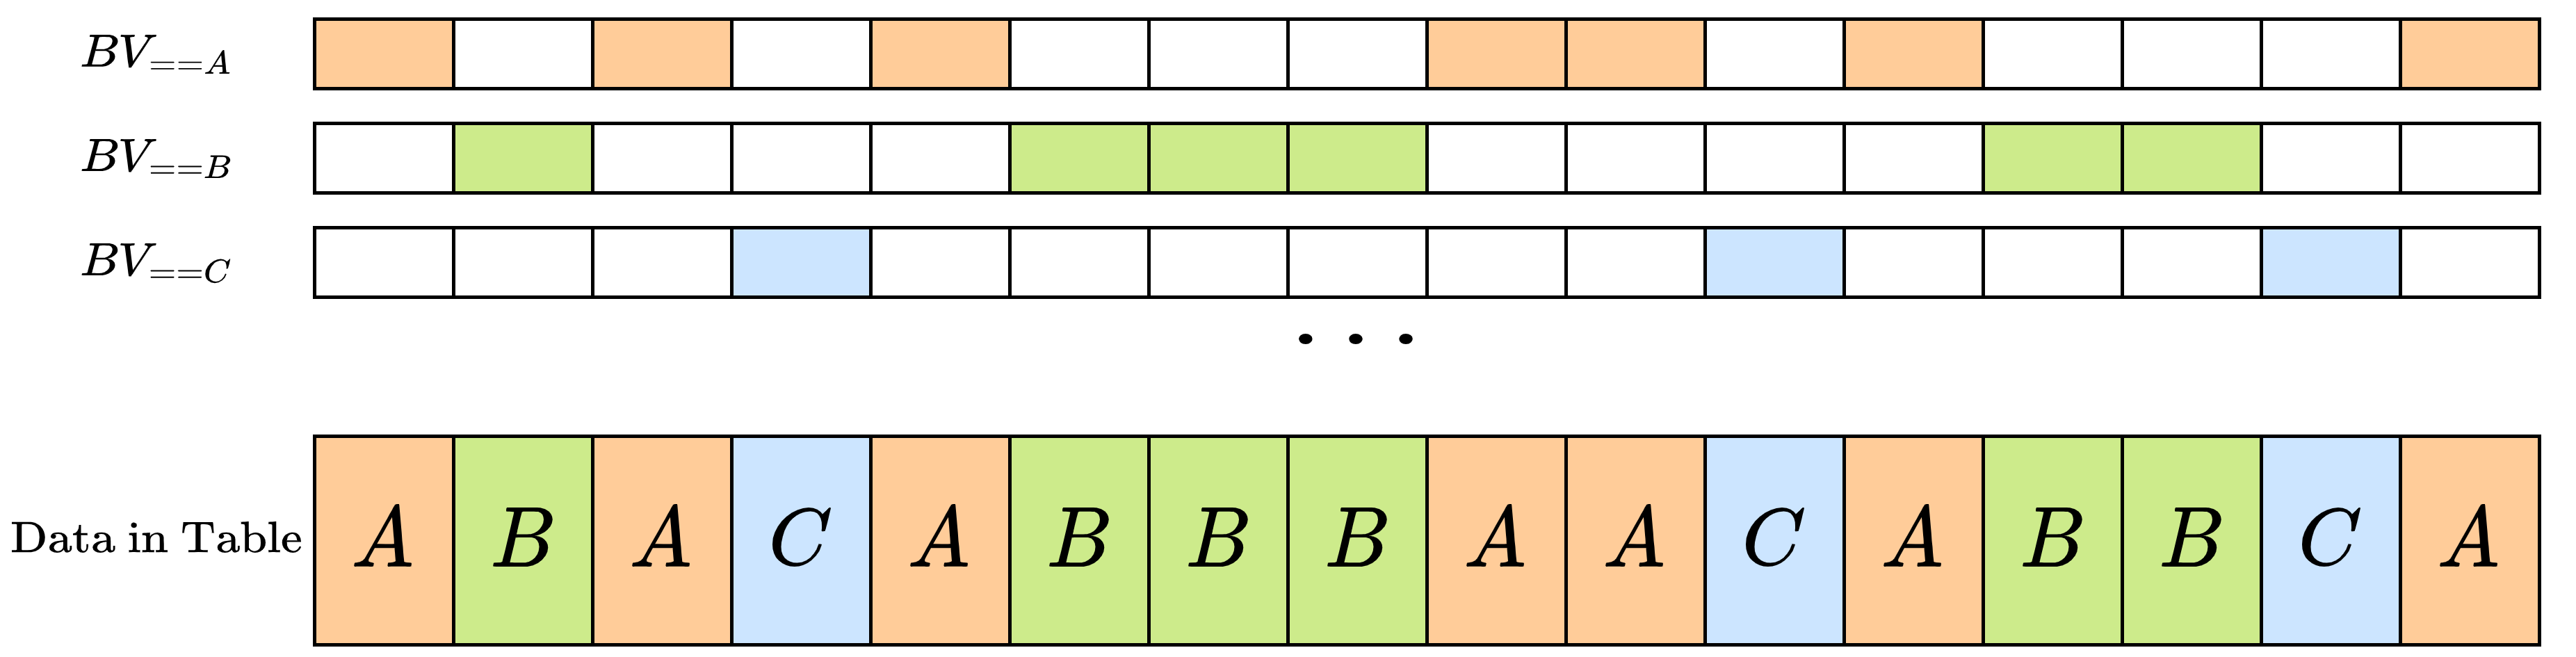
\includegraphics[width=.8\textwidth]{algorithms_and_indices/images/bitmap_index.drawio.png}
    \end{center}
    A collection of bitvectors on a column (each for a distinct value in the column).
    \begin{itemize}
        \item Need one bitvector per distinct value in the column
        \item Bitvectors usually disjoint (column can only be one distinct value at one time)
    \end{itemize}
    \[size(rows, distinct\_values) = \cfrac{rows \times distinct\_values}{8} \ bytes\]
\end{definitionbox}
On some systems we can create an index of arbitrary predicates, and to scan multiple bitmaps (using boolean operators on them).
\\
\\ The CPU operates in word size chunks of the bitvector. Hence we can easily check if all bits in a word size chunk (e.g 32 bits) are zero. We only need to iterate through this chunk if the chunk is non-zero.
\begin{minted}{cpp}
#include <cstddef>
#include <cstdint>
#include <iostream>
#include <vector>

using namespace std;

// scans a vector of 32 bit ints:
// - indexes each integer from LSB(0) to MSB(31)
// - does not consider endian-ness
// 100... 100... <=> [1,1]
vector<size_t> scan_bitmap(const vector<uint32_t> &bitvector) {
  vector<size_t> positions;
  size_t index = 0;
  for (auto elem : bitvector) {
    for (size_t small_index = 0; elem; small_index++, elem >>= 1) {
      if (elem & 1) {
        positions.push_back(index + small_index);
      }
    }
    index += 32;
  }
  return positions;
}
\end{minted}

\begin{tabbox}{prosbox}
    \textbf{Bandwidth} & Can scan a column with reduce memory bandwidth (e.g integers $\to$ bitmap index is $32$ times less). \\
    \textbf{Flexibility} & Can often use arbitrary predicates (e.g $< x$) to either turn a filter into a bitmap scan, or reduce time to scan (if $x < y$ an index $< x$ and help with a $< y$ filter). \\
\end{tabbox}

\subsubsection{Binned Bitmaps}
When there is are a high number of distinct values, but we do not want many bitvectors, we can create several bitvectors covering ranges of values.
\begin{itemize}
    \item The bitvectors ranges need to cover the entire domain.
    \item Smaller range $\to$ more precise and more useful for queries concerning data in that range, at the cost of more space used (more bitvectors)
    \item Not all ranges need to be the ame size, we can use the distribution of values to determine the ranges of the bins.
\end{itemize}
The \textit{false-positive rate} given a filter for $z$, and a bin of range $(x,y)$ where $x < x < y$, what proportion of the $1$s in the bitvector are not for the value $z$.
\begin{tcbraster}[raster columns=2, raster equal height]
    \begin{definitionbox}{Equi-Width}
        \[width = \cfrac{max(column) - min(column)}{number\_bins}\]
        Split range into several equal size bins. Useful for uniformly distributed (or near) data.
    \end{definitionbox}
    \begin{definitionbox}{Height Binning}
        All bins should contain the same number of values.
        \begin{itemize}
            \item Construction difficult (usually sort, determine quatiles on a sample)
            \item False-positive rate is value independent
            \item As table changes, may need to re-bin.
        \end{itemize}
    \end{definitionbox}
\end{tcbraster}

\subsubsection{Run Length Encoding}
\begin{center}
    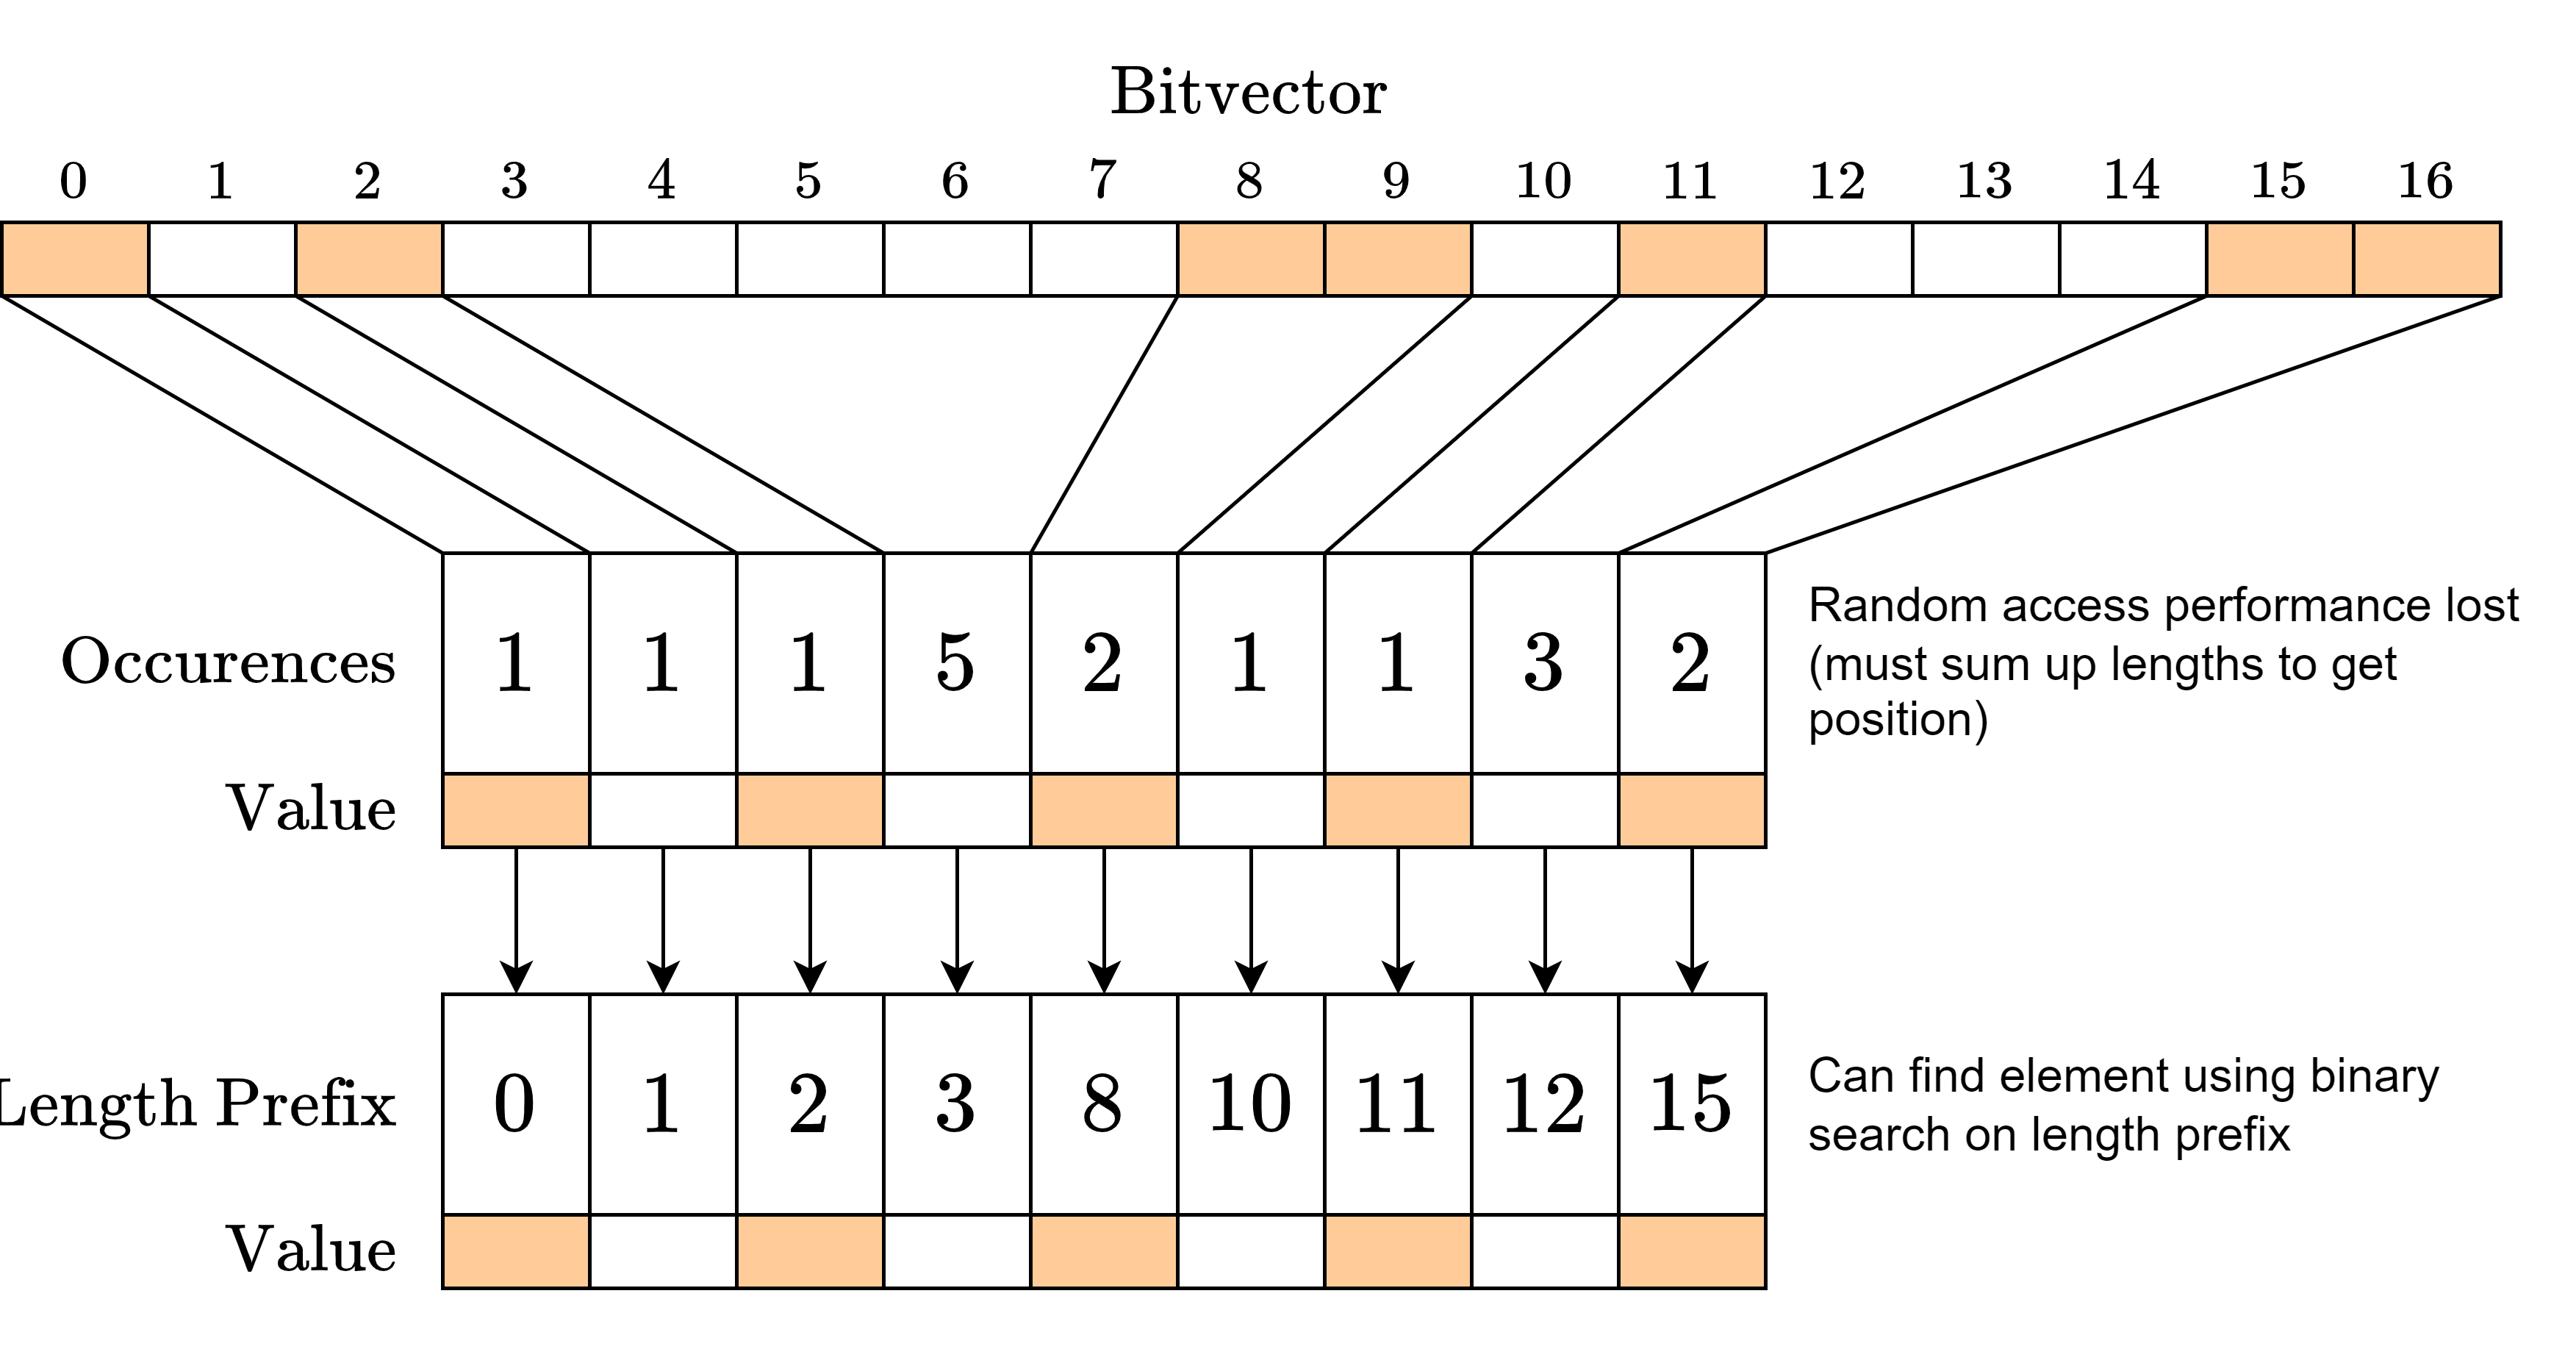
\includegraphics[width=.8\textwidth]{algorithms_and_indices/images/rle.drawio.png}
\end{center}

\subsection{B-Trees}
Trees are well suited to the requirements of a database:
\begin{itemize}
    \item Good complexity for equality lookups ($\log(n)$ tree traversal)
    \item Easy to update (hash-tables can require a resize and cause a load spike on insert)
\end{itemize}
Typical balanced tree data structures such as red/black trees, AVL trees are unsuited as they have low fan-out (require a large number of traversals to node spread across many pages $\to$ many page faults occur to fetch only a few nodes). Databases are I/O bound (here the I/O is page faults).

\begin{definitionbox}{B-Tree}
    \begin{center}
        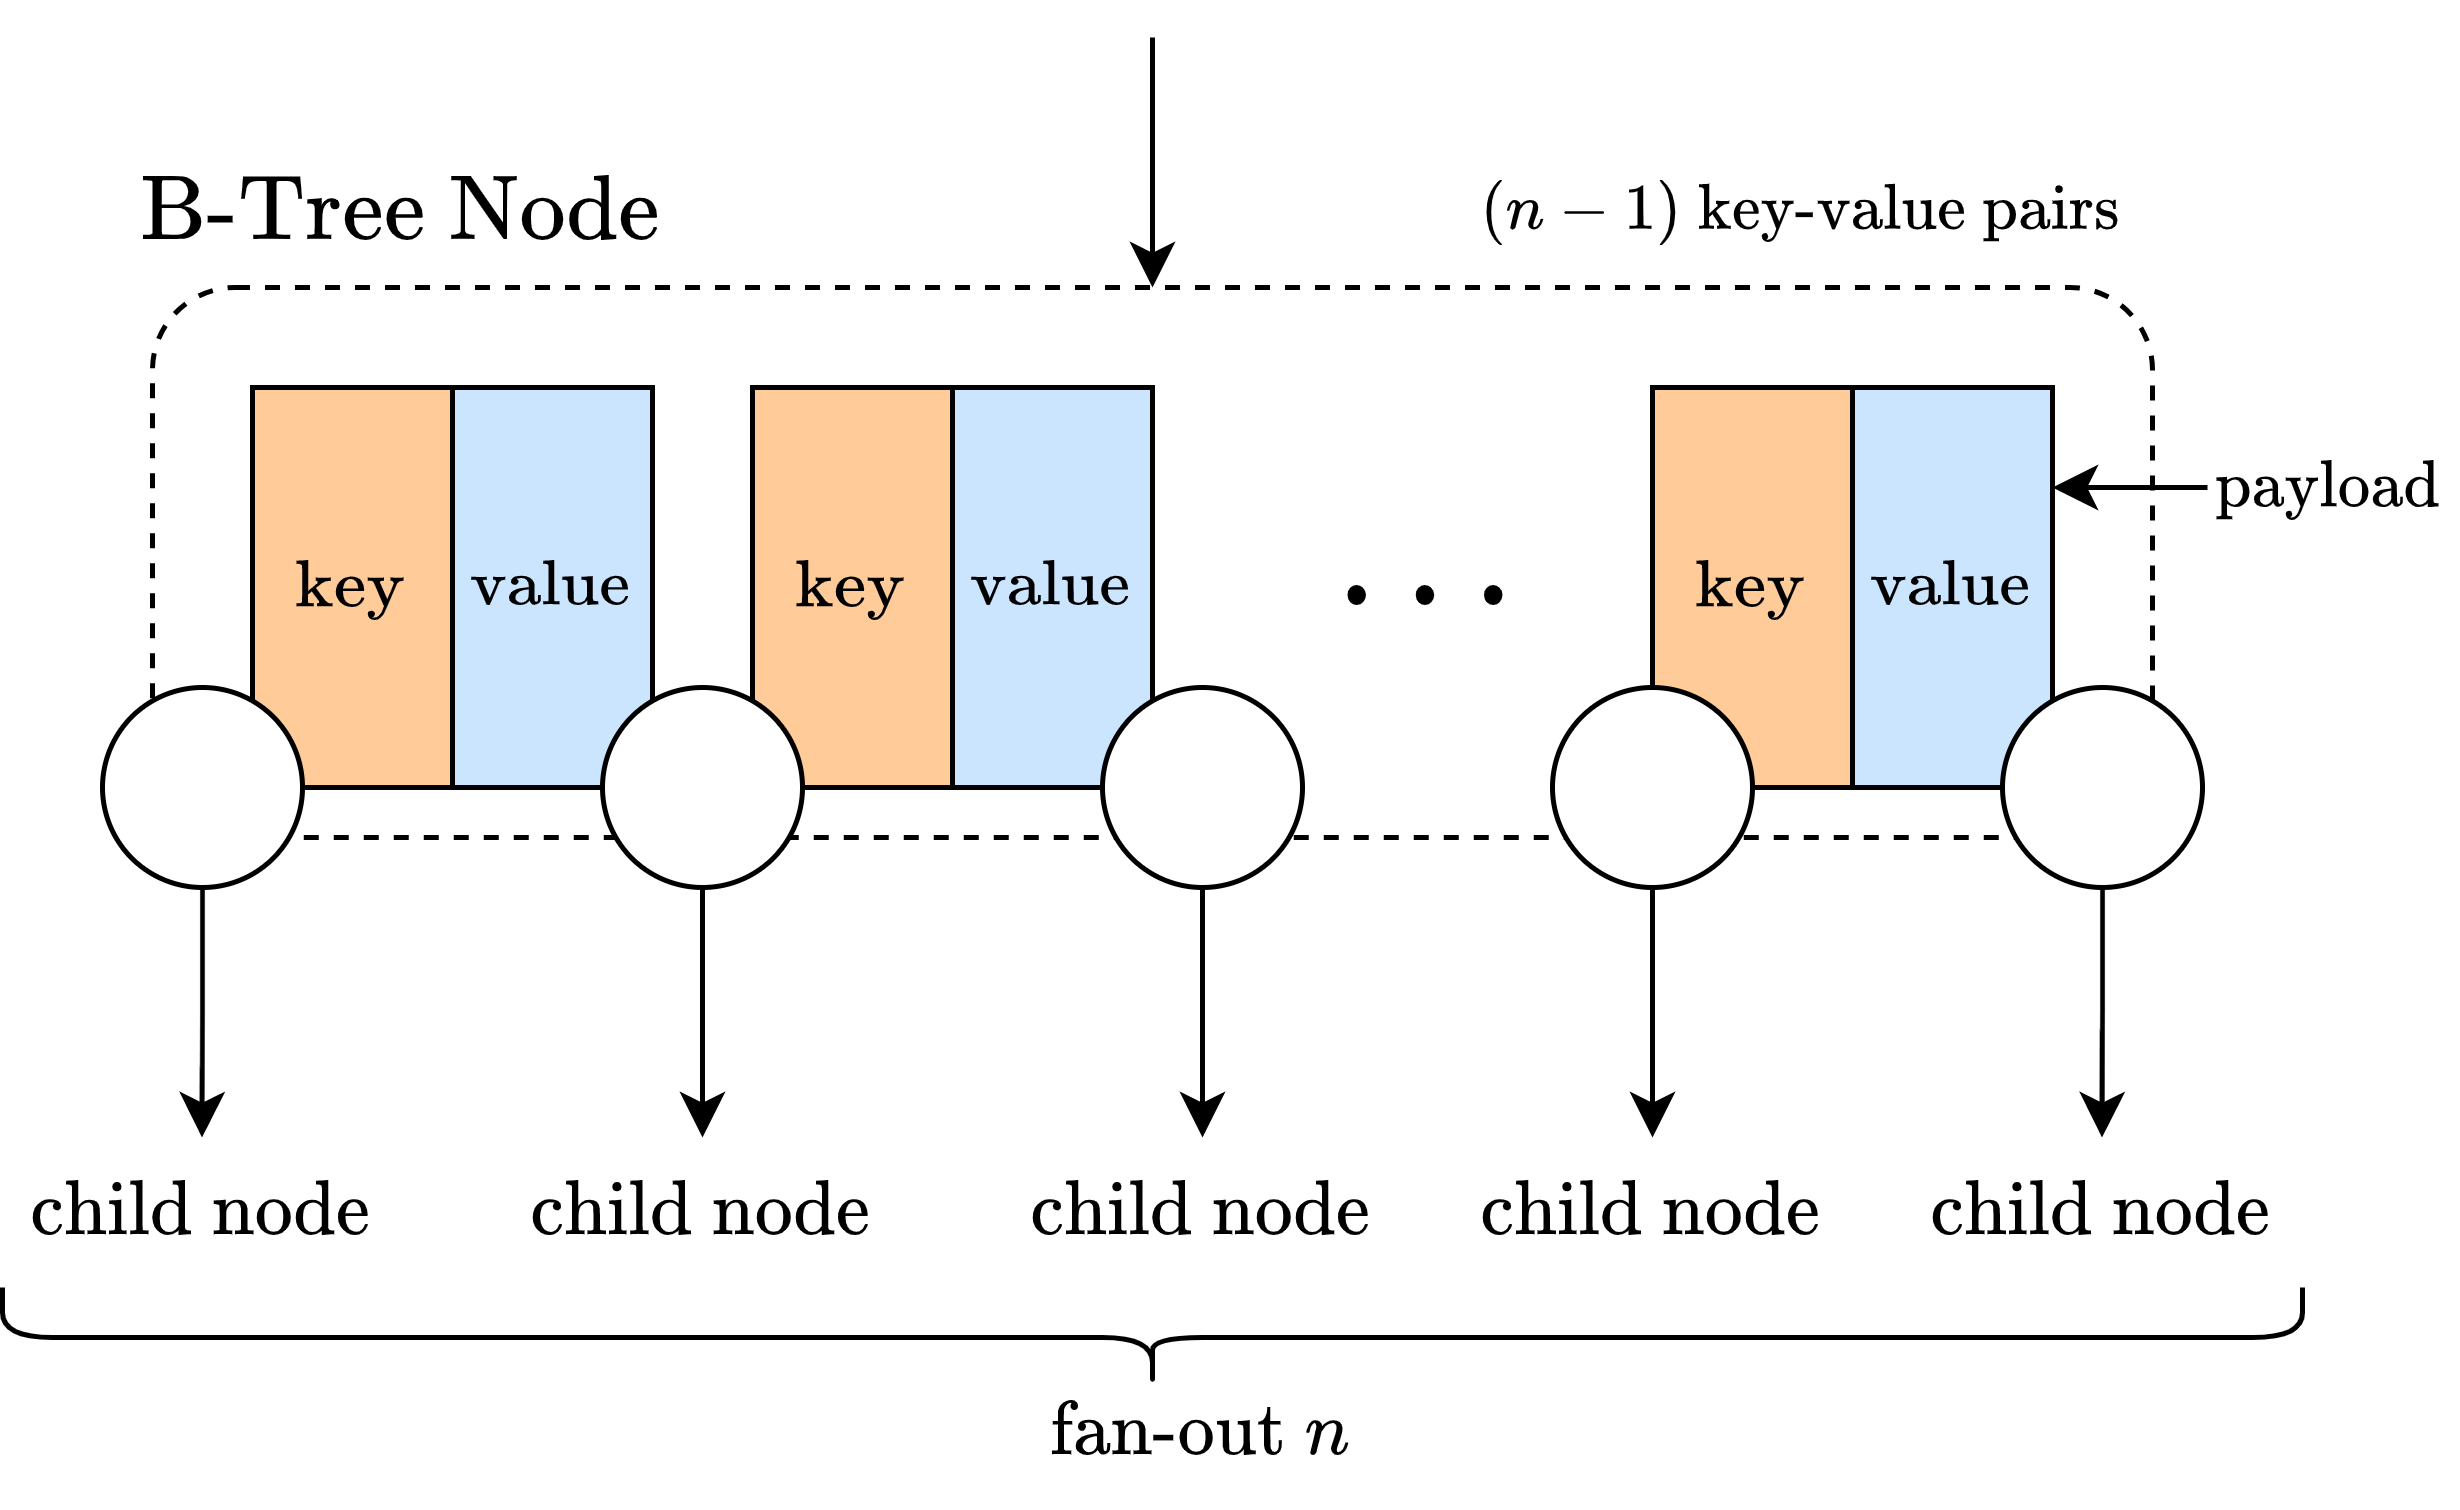
\includegraphics[width=.8\textwidth]{algorithms_and_indices/images/b_tree_node.drawio.png}
    \end{center}
    A high fan-out, balanced tree.
    \begin{itemize}
        \item Each non-root node must contain at least $\left\lfloor \cfrac{n-1}{2} \right\rfloor$ key/value pairs.
        \item The tree is kept balanced (all leaves at same depth)
        \item Time complexity for search, insert and delete is $O(\log n)$
    \end{itemize}
\end{definitionbox}

\subsection{B+ Trees}
\unfinished

\subsubsection{Maintaining Balance}
When a node overflows (full but value needs to be inserted), choose a splitting element and split values one either side into new nodes.
\\ \unfinished

\subsection{Foreign Key Indices}
Most joins are using a foreign key relation.
\begin{itemize}
    \item Constraint implies the number of matching tuples is 1 (foreign key $\to$ unique primary key)
    \item A foreign key indices effectively cache/save a join.
\end{itemize}
